\section{Memory Management}

\begin{frame}
  \frametitle{Physical and Virtual Memory}
  \begin{center}
    \includegraphics[height=0.8\textheight]{slides/kernel-driver-development-memory/mmu.pdf}
  \end{center}
\end{frame}

\begin{frame}
  \frametitle{Virtual Memory Organization}
  \begin{columns}
    \column{0.3\textwidth}
    \includegraphics[height=0.8\textheight]{slides/kernel-driver-development-memory/memory-organization.pdf}
    \column{0.7\textwidth}
    \begin{itemize}
    \item 1GB reserved for kernel-space
      \begin{itemize}
      \item Contains kernel code and core data structures, identical
        in all address spaces
      \item Most memory can be a direct mapping of physical memory at
        a fixed offset
      \end{itemize}
    \item Complete 3GB exclusive mapping available for each user space
      process
      \begin{itemize}
      \item Process code and data (program, stack, ...)
      \item Memory-mapped files
      \item Not necessarily mapped to physical memory (demand fault
        paging used for dynamic mapping to physical memory pages)
      \item Differs from one address space to another
      \end{itemize}
    \end{itemize}
  \end{columns}
\end{frame}

\begin{frame}
  \frametitle{Physical / virtual memory mapping}
  \begin{center}
    \includegraphics[height=0.8\textheight]{slides/kernel-driver-development-memory/memory-mapping.pdf}
  \end{center}
\end{frame}

\begin{frame}
  \frametitle{Accessing more physical memory}
  \begin{itemize}
  \item Only less than 1GB memory addressable directly through kernel
    virtual address space
  \item If more physical memory is present on the platform, part of
    the memory will not be accessible by kernel space, but can be used
    by user space
  \item To allow the kernel to access more physical memory:
    \begin{itemize}
    \item Change the 3GB/1GB memory split to 2GB/2GB or 1GB/3GB
      (\code{CONFIG_VMSPLIT_2G} or \code{CONFIG_VMSPLIT_1G)}
      $\Rightarrow$ reduce total user memory available for each process
    \item Change for a 64 bit architecture ;-) See
      \kerneldoctext{x86/x86_64/mm.txt} for an example.
    \item Activate \emph{highmem} support if available for your
      architecture:
      \begin{itemize}
      \item Allows kernel to map parts of its non-directly accessible
        memory
      \item Mapping must be requested explicitly
      \item Limited addresses ranges reserved for this usage
      \end{itemize}
    \end{itemize}
  \item See \url{http://lwn.net/Articles/75174/} for useful
    explanations
  \end{itemize}
\end{frame}

\begin{frame}
  \frametitle{Notes on user space memory}
  \begin{itemize}
  \item New user space memory is allocated either from the already
    allocated process memory, or using the \code{mmap} system call
  \item Note that memory allocated may not be physically allocated:
    \begin{itemize}
    \item Kernel uses demand fault paging to allocate the physical
      page (the physical page is allocated when access to the virtual
      address generates a page fault)
    \item ... or may have been swapped out, which also induces a page
      fault
    \end{itemize}
  \item User space memory allocation is allowed to over-commit memory
    (more than available physical memory) $\Rightarrow$ can lead to
    out of memory
  \item OOM killer kicks in and selects a process to kill to retrieve
    some memory.  That's better than letting the system freeze.
  \end{itemize}
\end{frame}

\begin{frame}
  \frametitle{Back to kernel memory}
  \begin{itemize}
  \item Kernel memory allocators (see following slides) allocate
    physical pages, and kernel allocated memory cannot be swapped out,
    so no fault handling required for kernel memory.
  \item Most kernel memory allocation functions also return a kernel
    virtual address to be used within the kernel space.
  \item Kernel memory low-level allocator manages pages. This is the
    finest granularity (usually 4 KB, architecture dependent).
  \item However, the kernel memory management handles smaller memory
    allocations through its allocator (see \emph{SLAB allocators}
    – used by \kfunc{kmalloc}).
  \end{itemize}
\end{frame}

\begin{frame}
  \frametitle{Allocators in the Kernel}
  \begin{center}
    \includegraphics[height=0.8\textheight]{slides/kernel-driver-development-memory/allocators.pdf}
  \end{center}
\end{frame}

\begin{frame}
  \frametitle{Page Allocator}
  \begin{itemize}
  \item Appropriate for medium-size allocations
  \item A page is usually 4K, but can be made greater in some
    architectures (sh, mips: 4, 8, 16 or 64 KB, but not configurable in
    x86 or arm).
  \item Buddy allocator strategy, so only allocations of power of two
    number of pages are possible: 1 page, 2 pages, 4 pages, 8 pages,
    16 pages, etc.
  \item Typical maximum size is 8192 KB, but it might depend on the
    kernel configuration.
  \item The allocated area is virtually contiguous (of course), but
    also physically contiguous. It is allocated in the identity-mapped
    part of the kernel memory space.
    \begin{itemize}
    \item This means that large areas may not be available or hard to
      retrieve due to physical memory fragmentation.
    \end{itemize}
  \end{itemize}
\end{frame}

\begin{frame}[fragile]
  \frametitle{Page Allocator API: Get free pages}
  \begin{itemize}
  \item \mint{c}+unsigned long get_zeroed_page(int flags)+
    \begin{itemize}
    \item Returns the virtual address of a free page, initialized to
      zero
    \item \code{flags}: see the next pages for details.
    \end{itemize}
  \item \mint{c}+unsigned long __get_free_page(int flags)+
    \begin{itemize}
    \item Same, but doesn't initialize the contents
    \end{itemize}
  \item \mint{c}+unsigned long __get_free_pages(int flags,+
    \mint{c}+unsigned int order)+
    \begin{itemize}
    \item Returns the starting virtual address of an area of several
      contiguous pages in physical RAM, with order being
      \code{log2(number_of_pages)}.Can be computed
      from the size with the \kfunc{get_order} function.
    \end{itemize}
  \end{itemize}
\end{frame}

\begin{frame}[fragile]
  \frametitle{Page Allocator API: Free Pages}
  \begin{itemize}
  \item \mint{c}+void free_page(unsigned long addr)+
    \begin{itemize}
    \item Frees one page.
    \end{itemize}
  \item \mint{c}+void free_pages(unsigned long addr,+
    \mint{c}+unsigned int order)+
    \begin{itemize}
    \item Frees multiple pages. Need to use the same order as in
      allocation.
    \end{itemize}
  \end{itemize}
\end{frame}

\begin{frame}
  \frametitle{Page Allocator Flags}
  The most common ones are:
  \begin{itemize}
  \item \ksym{GFP_KERNEL}
    \begin{itemize}
    \item Standard kernel memory allocation. The allocation may
      block in order to find enough available memory. Fine for most
      needs, except in interrupt handler context.
    \end{itemize}
  \item \ksym{GFP_ATOMIC}
    \begin{itemize}
    \item RAM allocated from code which is not allowed to block
      (interrupt handlers or critical sections). Never blocks,
      allows to access emergency pools, but can fail if no free
      memory is readily available.
    \end{itemize}
  \item \ksym{GFP_DMA}
    \begin{itemize}
    \item Allocates memory in an area of the physical memory usable
      for DMA transfers. See our DMA chapter.
    \end{itemize}
  \item Others are defined in \kfile{include/linux/gfp.h}
  \end{itemize}
\end{frame}

\begin{frame}
  \frametitle{SLAB Allocator 1/2}
  \begin{itemize}
  \item The SLAB allocator allows to create {\em caches}, which contain a
    set of objects of the same size
  \item The object size can be smaller or greater than the page size
  \item The SLAB allocator takes care of growing or reducing the size
    of the cache as needed, depending on the number of allocated
    objects. It uses the page allocator to allocate and free pages.
  \item SLAB caches are used for data structures that are present in
    many many instances in the kernel: directory entries, file
    objects, network packet descriptors, process descriptors, etc.
    \begin{itemize}
    \item See \code{/proc/slabinfo}
    \end{itemize}
  \item They are rarely used for individual drivers.
  \item See \kfile{include/linux/slab.h} for the API
\end{itemize}
\end{frame}

\begin{frame}
  \frametitle{SLAB Allocator 2/2}
  \begin{center}
    \includegraphics[height=0.8\textheight]{slides/kernel-driver-development-memory/slab-allocator.pdf}
  \end{center}
\end{frame}

\begin{frame}[fragile]
  \frametitle{Different SLAB Allocators}
  \small
  There are three different, but API compatible, implementations of
  a SLAB allocator in the Linux kernel. A particular implementation
  is chosen at configuration time.
  \begin{itemize}
  \item SLAB: legacy, well proven allocator.\\
        Linux 4.20 on ARM: used in 48 \code{defconfig} files
  \item SLOB: much simpler. More space efficient but doesn't scale
        well. Can save space in small systems (depends on
        \code{CONFIG_EXPERT}). \\
        Linux 4.20 on ARM: used in 7 \code{defconfig} files \\
        Results on BeagleBone Black: -5 KB compressed kernel size, +1.43 s boot time!
  \item SLUB: more recent and simpler than
        SLAB, scaling much better (in particular for huge systems) and
        creating less fragmentation.\\
        Linux 4.20 on ARM: used in 0 \code{defconfig} files \\
	Results on BeagleBone Black: +4 KB compressed kernel, + 2ms total boot time.
  \end{itemize}
  \begin{center}
    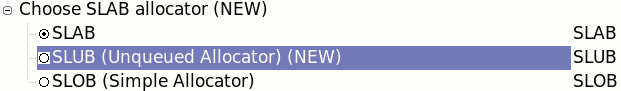
\includegraphics[height=0.2\textheight]{slides/kernel-driver-development-memory/slab-screenshot.png}
  \end{center}
\end{frame}

\begin{frame}
  \frametitle{kmalloc Allocator}
  \begin{itemize}
  \item The kmalloc allocator is the general purpose memory allocator
    in the Linux kernel
  \item For small sizes, it relies on generic SLAB caches, named
    \code{kmalloc-XXX} in \code{/proc/slabinfo}
  \item For larger sizes, it relies on the page allocator
  \item The allocated area is guaranteed to be physically contiguous
  \item The allocated area size is rounded up to the size of the
        smallest SLAB cache in which it can fit
        (while using the SLAB allocator directly allows to have more
        flexibility)
  \item It uses the same flags as the page allocator (\ksym{GFP_KERNEL},
    \ksym{GFP_ATOMIC}, \ksym{GFP_DMA}, etc.) with the same semantics.
  \item Maximum sizes, on \code{x86} and \code{arm} (see
    \url{http://j.mp/YIGq6W}): \\
    - Per allocation: 4 MB \\
    - Total allocations: 128 MB
  \item Should be used as the primary allocator unless there is a
    strong reason to use another one.
  \end{itemize}
\end{frame}

\begin{frame}[fragile]
  \frametitle{kmalloc API 1/2}
  \begin{itemize}
  \item \mint{c}+#include <linux/slab.h>+
  \item \mint{c}+void *kmalloc(size_t size, int flags);+
    \begin{itemize}
    \item Allocate \code{size} bytes, and return a pointer to the area
      (virtual address)
    \item \code{size}: number of bytes to allocate
    \item \code{flags}: same flags as the page allocator
    \end{itemize}
  \item \mint{c}+void kfree(const void *objp);+
    \begin{itemize}
    \item Free an allocated area
    \end{itemize}
  \item Example: (\kfile{drivers/infiniband/core/cache.c})
\begin{minted}{c}
struct ib_update_work *work;
work = kmalloc(sizeof *work, GFP_ATOMIC);
...
kfree(work);
\end{minted}
  \end{itemize}
\end{frame}

\begin{frame}[fragile]
  \frametitle{kmalloc API 2/2}
  \begin{itemize}
  \item \mint{c}+void *kzalloc(size_t size, gfp_t flags);+
    \begin{itemize}
    \item Allocates a zero-initialized buffer
    \end{itemize}
  \item \mint{c}+void *kcalloc(size_t n, size_t size, gfp_t flags);+
    \begin{itemize}
    \item Allocates memory for an array of \code{n} elements of
      \code{size} size, and zeroes its contents.
    \end{itemize}
  \item {\footnotesize \mint{c}+void *krealloc(const void *p, size_t new_size, gfp_t flags);+}
    \begin{itemize}
    \item Changes the size of the buffer pointed by \code{p} to
      \code{new_size}, by reallocating a new buffer and copying the
      data, unless \code{new_size} fits within the alignment of
      the existing buffer.
    \end{itemize}
  \end{itemize}
\end{frame}

\begin{frame}
  \frametitle{devm\_ kmalloc functions}
  Allocations with automatic freeing when the corresponding device or module is unprobed.
  \begin{itemize}
  \scriptsize
  \item \mint{c}+void *devm_kmalloc(struct device *dev, size_t size, int flags);+
  \item \mint{c}+void *devm_kzalloc(struct device *dev, size_t size, int flags);+
  \item \mint{c}+void *devm_kcalloc(struct device *dev, size_t n, size_t size, gfp_t flags);+
  \item \mint{c}+void *devm_kfree(struct device *dev, void *p);+
        Useful to immediately free an allocated buffer
  \end{itemize}
  \normalsize
  For use in \code{probe()} functions.
\end{frame}

\begin{frame}[fragile]
  \frametitle{vmalloc Allocator}
  \begin{itemize}
  \item The \kfunc{vmalloc} allocator can be used to obtain virtually
    contiguous memory zones, but not physically contiguous. The
    requested memory size is rounded up to the next page.
  \item The allocated area is in the kernel space part of the address
    space, but outside of the identically-mapped area
  \item Allocations of fairly large areas is possible (almost as big
    as total available memory, see \url{http://j.mp/YIGq6W} again),
    since physical memory fragmentation is not an issue, but areas
    cannot be used for DMA, as DMA usually requires physically
    contiguous buffers.
  \item Example use: to allocate kernel buffers to load module code.
  \item API in \kfile{include/linux/vmalloc.h}
    \begin{itemize}
    \item \mint{c}+void *vmalloc(unsigned long size);+
      \begin{itemize}
      \item Returns a virtual address
      \end{itemize}
    \item \mint{c}+void vfree(void *addr);+
    \end{itemize}
  \end{itemize}
\end{frame}

\begin{frame}
  \frametitle{Kernel memory debugging}
  \begin{itemize}
  \item \code{KASAN}
    \begin{itemize}
    \item Dynamic memory error detector, to find use-after-free and
      out-of-bounds bugs.
    \item Only available on \code{x86_64}, \code{arm64}, \code{s390} and
      \code{xtensa} so far (Linux 4.20 status), but will help to improve
      architecture independent code anyway.
    \item See \kerneldochtml{dev-tools/kasan} for details.
    \end{itemize}
  \item \code{Kmemleak}
    \begin{itemize}
    \item Dynamic checker for memory leaks
    \item This feature is available for all architectures.
    \item See \kerneldochtml{dev-tools/kmemleak} for details.
    \end{itemize}
  \end{itemize}
  Both have a significant overhead. Only use them in development!
\end{frame}

\begin{frame}
  \frametitle{Kernel memory management: resources}
  Virtual memory and Linux, Alan Ott and Matt Porter, 2016\\
  Great and much more complete presentation about this topic\\
  \url{http://bit.ly/2Af1G2i} (video: \url{http://bit.ly/2Bwwv0C})
  \begin{center}
     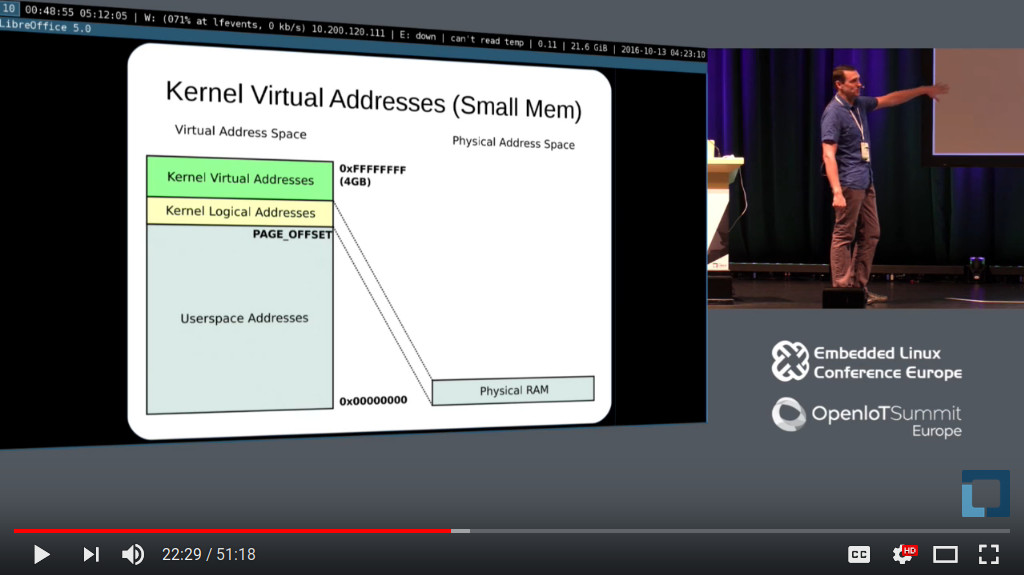
\includegraphics[height=0.6\textheight]{slides/kernel-driver-development-memory/ott-porter-kernel-virtual-memory-presentation.jpg}
  \end{center}
\end{frame}
